% latex presentation
\documentclass[pdf]{beamer}
\usetheme{CambridgeUS}
\setbeamersize{text margin left=20pt, text margin right=20pt}
\setbeamertemplate{navigation symbols}{}

% english document
\usepackage[utf8]{inputenc}
\usepackage[american]{babel}

% images
\graphicspath{{../latex/}}

% units and nice numbers
\usepackage[group-separator={,}]{siunitx}

% fancy author: https://tex.stackexchange.com/questions/271433/thesis-title-slide
\newsavebox{\authbox}
\sbox{\authbox}{
    \centering
    \begin{minipage}{0.45\linewidth}
        \centering
        \normalsize
        {\footnotesize Advisor}
        \par
        Alberto Montresor
    \end{minipage}
    \hfill
    \begin{minipage}{0.45\linewidth}
        \centering
        \normalsize
        {\footnotesize Student}
        \par
        Davide Pedranz
    \end{minipage}
}

% fancy date
\newsavebox{\instbox}
\sbox{\instbox}{
    \centering
    \begin{minipage}{\linewidth}
        \centering
        \normalsize
        \vspace{4mm}
        \small
        University of Trento
        \par
        \vspace{0.5mm}
        \footnotesize Department of Information Engineering and Computer Science
        \vspace{4mm}
    \end{minipage}
}

% thesis details
\title[Final Dissertation]{Final Dissertation}
\subtitle{Simulating large-scale network attacks against Bitcoin}
\author[Davide Pedranz]{\usebox{\authbox}}
\institute[]{\usebox{\instbox}}
\date[10 October 2018]{\footnotesize 10 October 2018}

% slides
\begin{document}

\begin{frame}
	\titlepage
\end{frame}

\begin{frame}
	\frametitle{Outline}
	\tableofcontents[pausesections]
\end{frame}


\AtBeginSection[]
{
	\begin{frame}<beamer>
		\frametitle{Outline}
		\tableofcontents[currentsection]
	\end{frame}
}

\section{Bitcoin}

\subsection*{Introduction}
\begin{frame}
	\frametitle{Bitcoin}
	\begin{columns}
		\column{0.7\textwidth}
		\begin{itemize}
			\setlength \itemsep{1.5em}
			\item<1-> Most used and valuable cryptocurrency:
			\begin{itemize}
				\item<1-> Price = $\sim$ 8000 \$/BTC
				\item<1-> Market cap = $\sim$ 141 billion \$
			\end{itemize}
			\item<2-> Usages:
			\begin{itemize}
				\item<2-> in-shop payments
				\item<2-> online purchases
				\item<2-> low-cost money transfer
			\end{itemize}
		\end{itemize}
		\column{0.3\textwidth}
		\begin{figure}
			\hspace*{-1cm}
			
\includegraphics[width=0.9\columnwidth]{figures/bitcoin}
			\vspace*{-0.1cm}
		\end{figure}
	\end{columns}
\end{frame}

\subsection{Blockchain}
\begin{frame}
	\frametitle{Blockchain}
	\begin{figure}
		\centering
		\vspace*{0.5cm}
		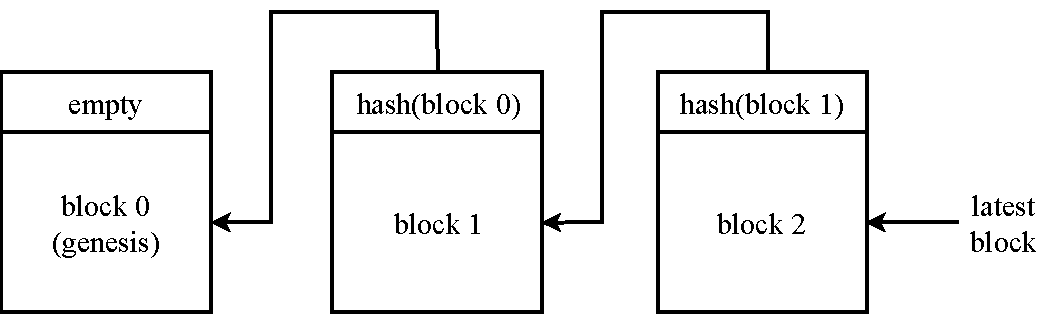
\includegraphics[width=\columnwidth]{figures/blockchain}
		\vspace*{0.5cm}
		\caption{
			Schematic representation of a blockchain.
			A blockchain is a list of blocks, connected to each other with an hash pointer.
			Each block contains a set of transactions.
		}
	\end{figure}
\end{frame}

\subsection{Forks}
\begin{frame}
	\frametitle{Forks}
	\begin{overprint}
		\onslide<1>
		\begin{figure}
			\centering
			\vspace*{0.5cm}
			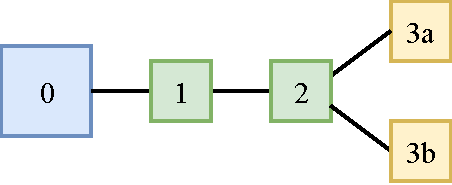
\includegraphics[scale=0.9]{figures/forks_1}
			\vspace*{0.5cm}
			\caption{
				Schematic representation of a blockchain with \num{2} branches.
				The yellow blocks \texttt{3a} and \texttt{3b} are in conflict.
				The network will pick only one of them.
			}
		\end{figure}
		\onslide<2>
		\begin{figure}
			\centering
			\vspace*{0.5cm}
			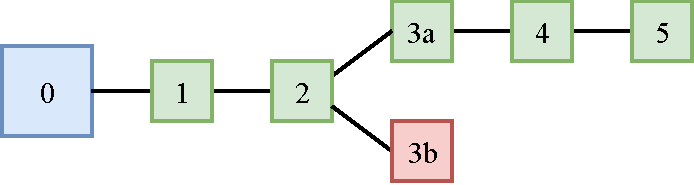
\includegraphics[scale=0.9]{figures/forks_2}
			\vspace*{0.5cm}
			\caption{
				Schematic representation of a blockchain with one fork.
				The green block are on the longest chain.
				The red block \texttt{3b} is in conflict with \texttt{3a}.
			}
		\end{figure}
	\end{overprint}
\end{frame}

\subsection{Mining}
\begin{frame}
	\frametitle{Mining}
	Mining is the process of creating new blocks:
	\begin{itemize}
		\item each valid block contains the solution of a computational puzzle
		\item the only known way to solve the puzzle is the brute-force approach
		\item the puzzle's solution proves that some work has been done
		\item the miner receives a reward for each completed valid block on the longest chain
	\end{itemize}
				
	\par
	\vspace{5mm}
	\textit{Proof-of-Work} prevents attackers to generate too many valid blocks.
\end{frame}

\section{Attacks}
\subsection{Double Spending}
\begin{frame}
	\frametitle{Double Spending}
	\begin{overprint}
		\onslide<1>
		\begin{figure}
			\centering
			\vspace*{0.1cm}
			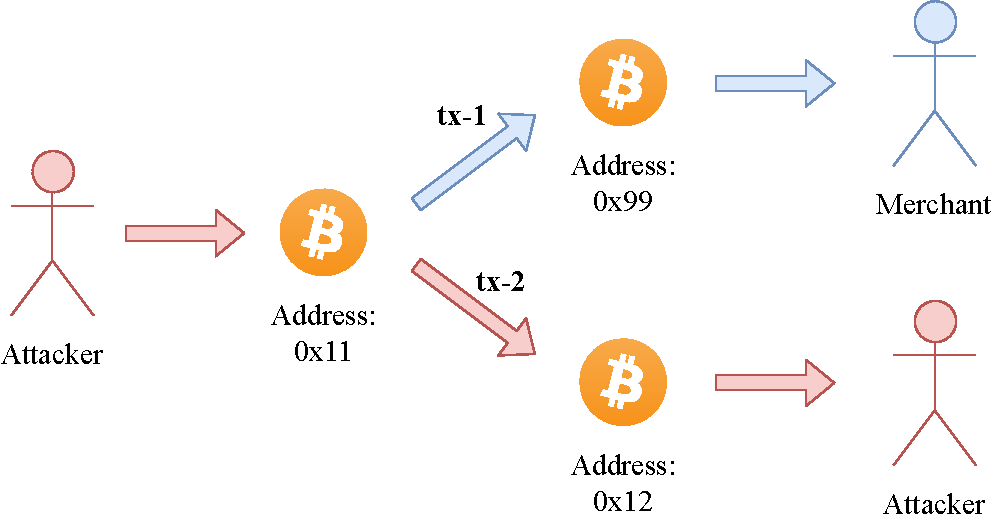
\includegraphics[width=0.9\columnwidth]{figures/race_attack_2}
			\vspace*{0.2cm}
			\caption{
				The attacker submits the transaction \texttt{tx-1} to pay the merchant.
				At the same time, it submits the conflicting transaction \texttt{tx-2}.
			}
		\end{figure}
		\onslide<2>
		\begin{figure}
			\centering
			\vspace*{0.1cm}
			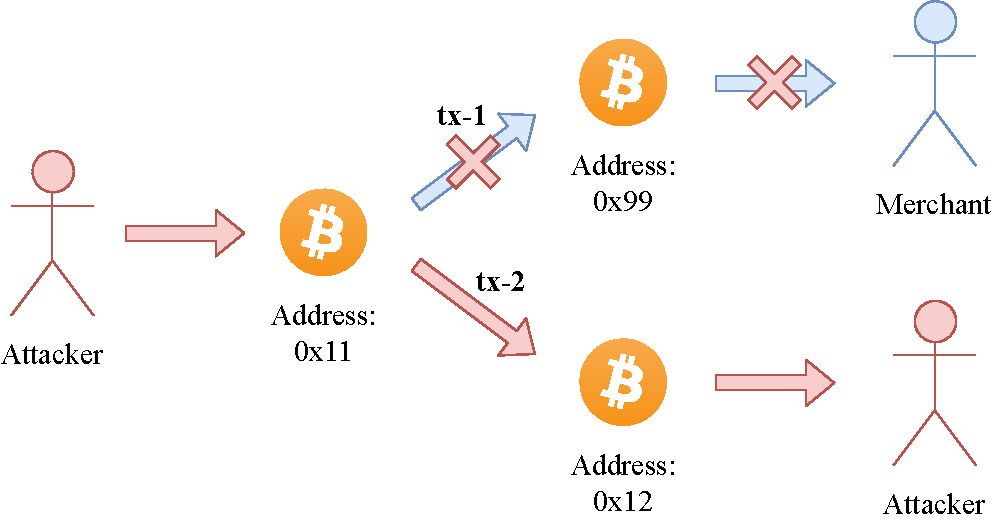
\includegraphics[width=0.9\columnwidth]{figures/race_attack_3}
			\vspace*{0.2cm}
			\caption{
				The transaction \texttt{tx-2} is accepted, \texttt{tx-1} is rejected.
				The attacker gets its money back, while the merchant does not get anything.
			}
		\end{figure}
	\end{overprint}
\end{frame}

\subsection{Balance Attack}
\begin{frame}
	\frametitle{Balance Attack}
	\begin{columns}
		\column{0.5\textwidth}
		The attacker:
		\begin{itemize}
			\item partitions the nodes into groups with about the same computational power
			\item delays or drops messages between nodes in different groups
		\end{itemize}
																																
		\column{0.5\textwidth}
		\centering
		\hspace*{-3mm}										
		\begin{figure}
			\begin{overprint}
				\onslide<1>
				\hspace{1.4mm}
				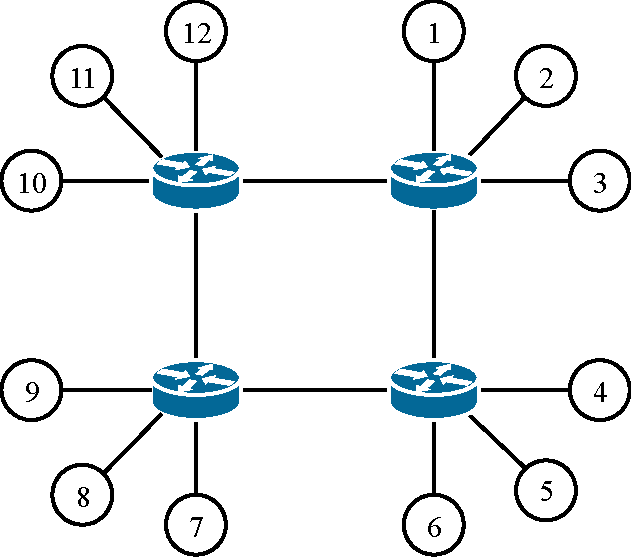
\includegraphics[scale=0.5]{figures/balance_1}
				\onslide<2>
				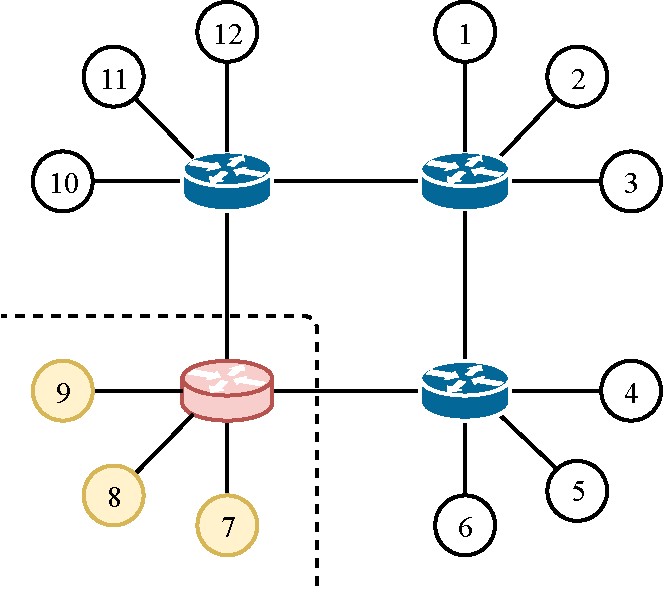
\includegraphics[scale=0.5]{figures/balance}
			\end{overprint}
		\end{figure}
	\end{columns}
\end{frame}

\section{Experiments}
\subsection*{Simulator}
\begin{frame}
	\frametitle{Simulator}
	\begin{itemize}
		\setlength \itemsep{1.5em}
		\item Bitcoin protocol:
		      \begin{itemize}
		      	\setlength \itemsep{0.5em}
		      	\item network bootstrap
		      	\item topology construction
		      	\item blocks and transactions propagation
		      \end{itemize}
		\item Simulate the Balance Attack for different:
		      \begin{itemize}
		      	\setlength \itemsep{0.5em}
		      	\item delays
		      	\item drops
		      	\item partitions
			  \end{itemize}
		\item Evaluation metric: number of forks
	\end{itemize}
\end{frame}

\subsection{Delay}
\begin{frame}
	\frametitle{Balance Attack with Delays}
	\begin{figure}
		\centering
		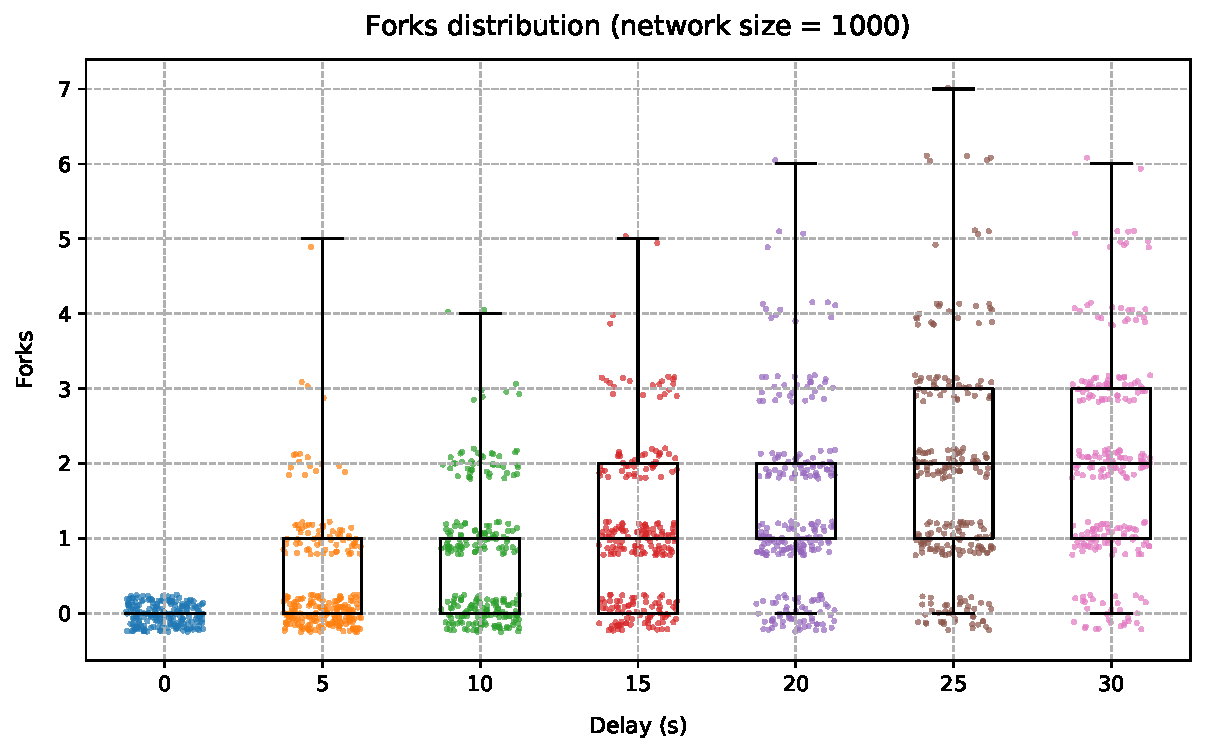
\includegraphics[width=\columnwidth]{plots/forks_attack_delay_1000_boxplot_1}
	\end{figure}
\end{frame}
\begin{frame}
	\frametitle{Balance Attack with Delays for Different Networks}
	\begin{figure}
		\centering
		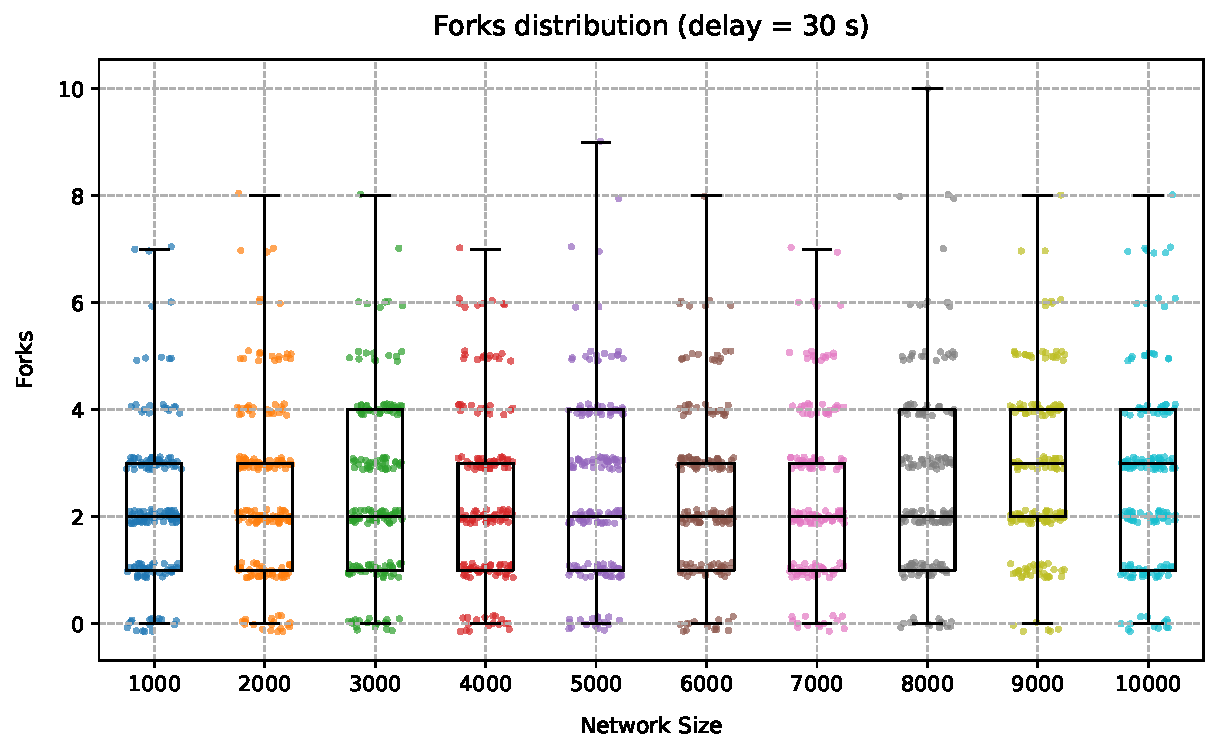
\includegraphics[width=\columnwidth]{plots/forks_attack_delay_30_network_sizes_boxplot_1}
	\end{figure}
\end{frame}

\subsection{Drop}
\begin{frame}
	\frametitle{Balance Attack with Random Message Drop}
	\begin{figure}
		\centering
		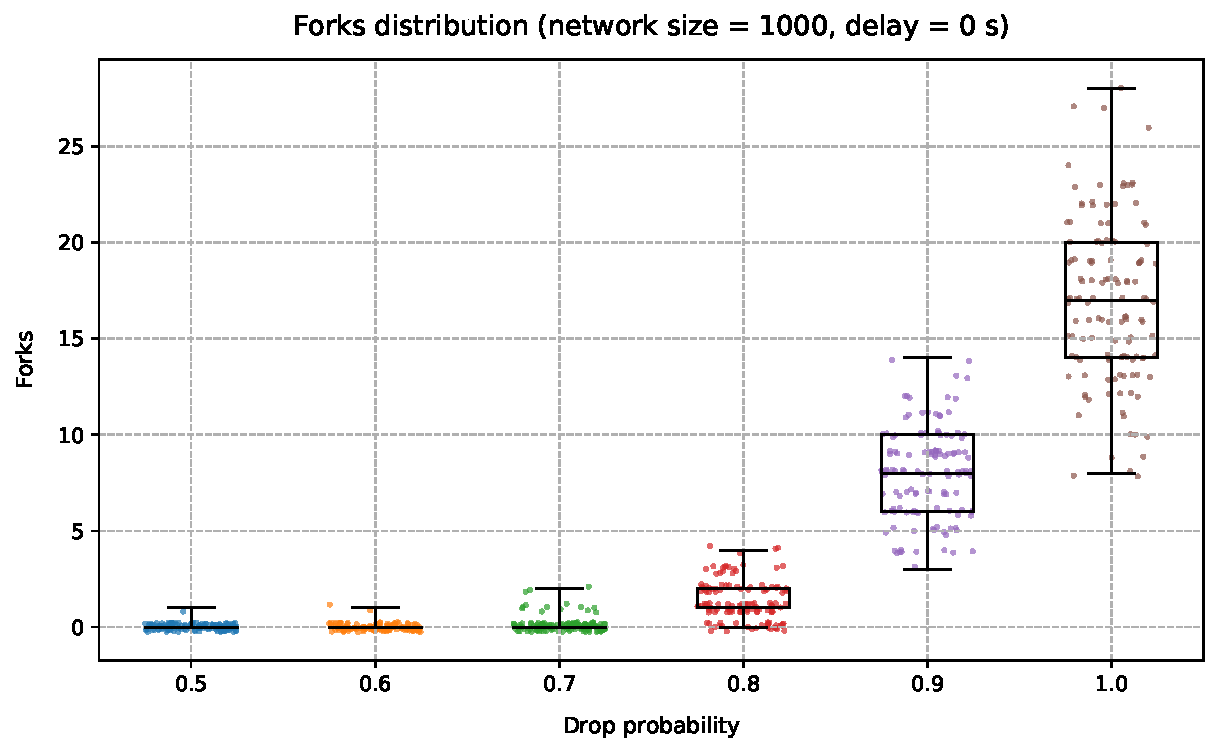
\includegraphics[width=\columnwidth]{plots/forks_attack_drop_boxplot_1}
	\end{figure}
\end{frame}

\subsection{Partition}
\begin{frame}
	\frametitle{Balance Attack with Multiple Groups}
	\begin{figure}
		\centering
		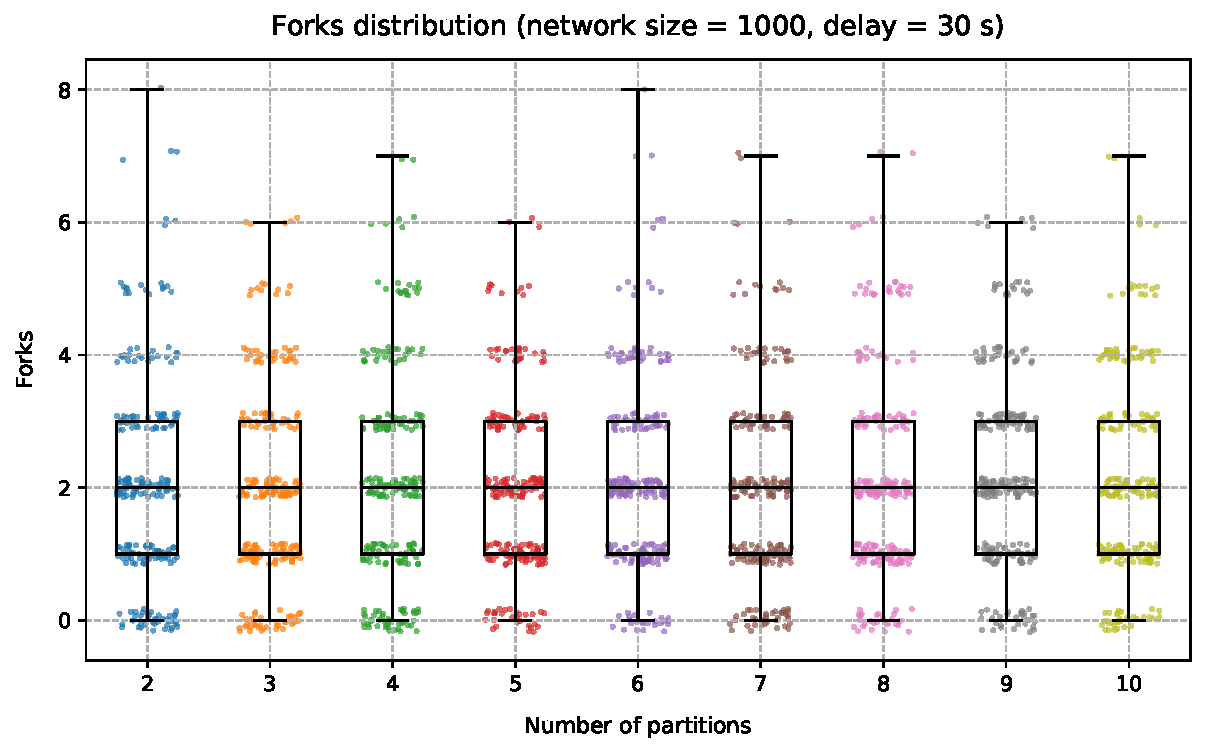
\includegraphics[width=\columnwidth]{plots/forks_attack_partitions_boxplot_1}
	\end{figure}
\end{frame}

\section{Conclusions}
\subsection*{Results}
\begin{frame}
	\frametitle{Conclusions}
	\begin{itemize}
		\setlength \itemsep{0.8em}
		\item<1-> Bitcoin behaves well under normal network conditions
		\item<2-> The Balance attack works and scales to different network sizes
		\item<3-> The Bitcoin protocol handles well the loss of many messages
		\item<4-> The number of groups does not affect the attack's performances 
	\end{itemize}
\end{frame}

\subsection*{Thanks}
\begin{frame}[c]{}
	\centering
	\vspace*{1.3cm}
	\Large Thanks for the attention!
\end{frame}

\end{document}
